\section{Tests of additional meta-parameters}
\lb{sec:app}

In this appendix we discuss tests of some meta-parameters, which had a relatively little effect on the 
accuracy of the algorithms. For these tests we use the 2-class classification in the 3FGL catalog.

For the LR algorithm, we test two additional meta-parameters: regularization and tolerance. 
The effect of the choice of these parameters on accuracy is less than 1\% (Fig. \ref{fig:LR_tol_reg}). 
Therefore we used the default values for these parameters (tolerance is $10^{-4}$ and regularization parameter is 1)
both in the 2-class and in the 3-class classifications.

\begin{figure}[h]
\centering
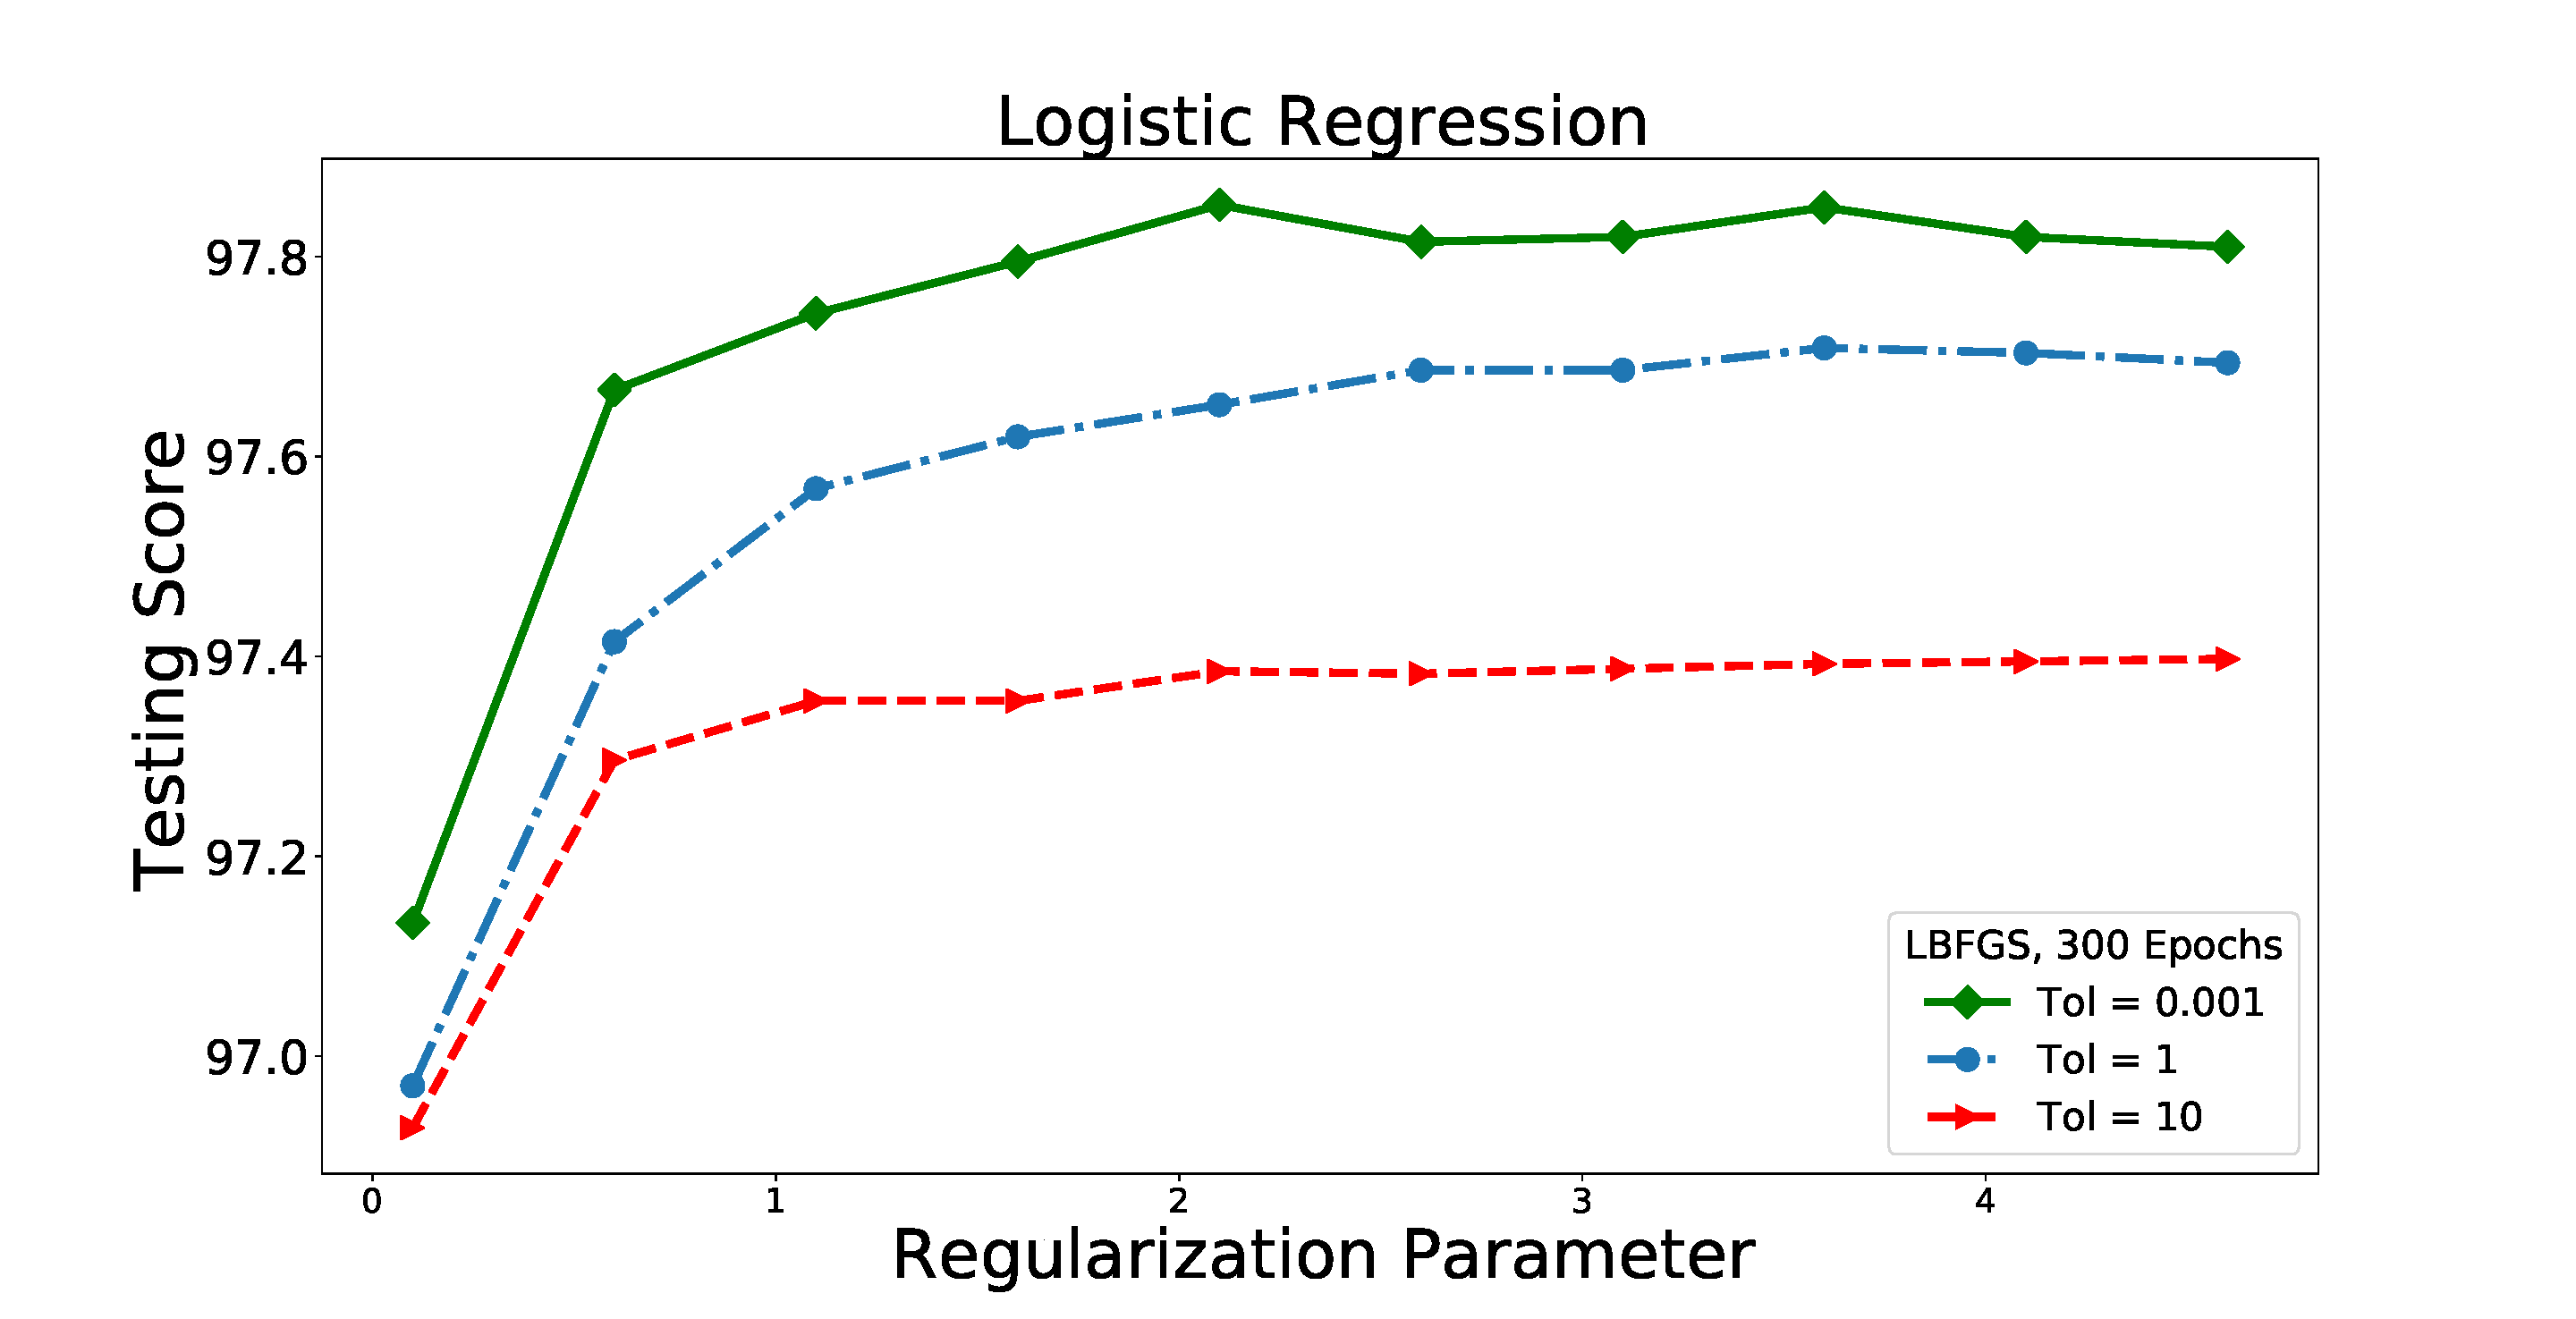
\includegraphics[width=\twopicsp\textwidth]{plots/lr_train_reg.pdf}
\caption{Dependence of LR on tolerance and regularization. 
}
\label{fig:LR_tol_reg}
\end{figure}

In Fig. \ref{fig:nn_nn} we show the effect of adding the second hidden layer in the NN algorithm.
The difference between the best accuracies of the NN with one hidden layer (cf. Table \ref{tab:selected_algs})
and  the NN with the additional hidden layer is less then 1\%.
\begin{figure}[h]
\centering
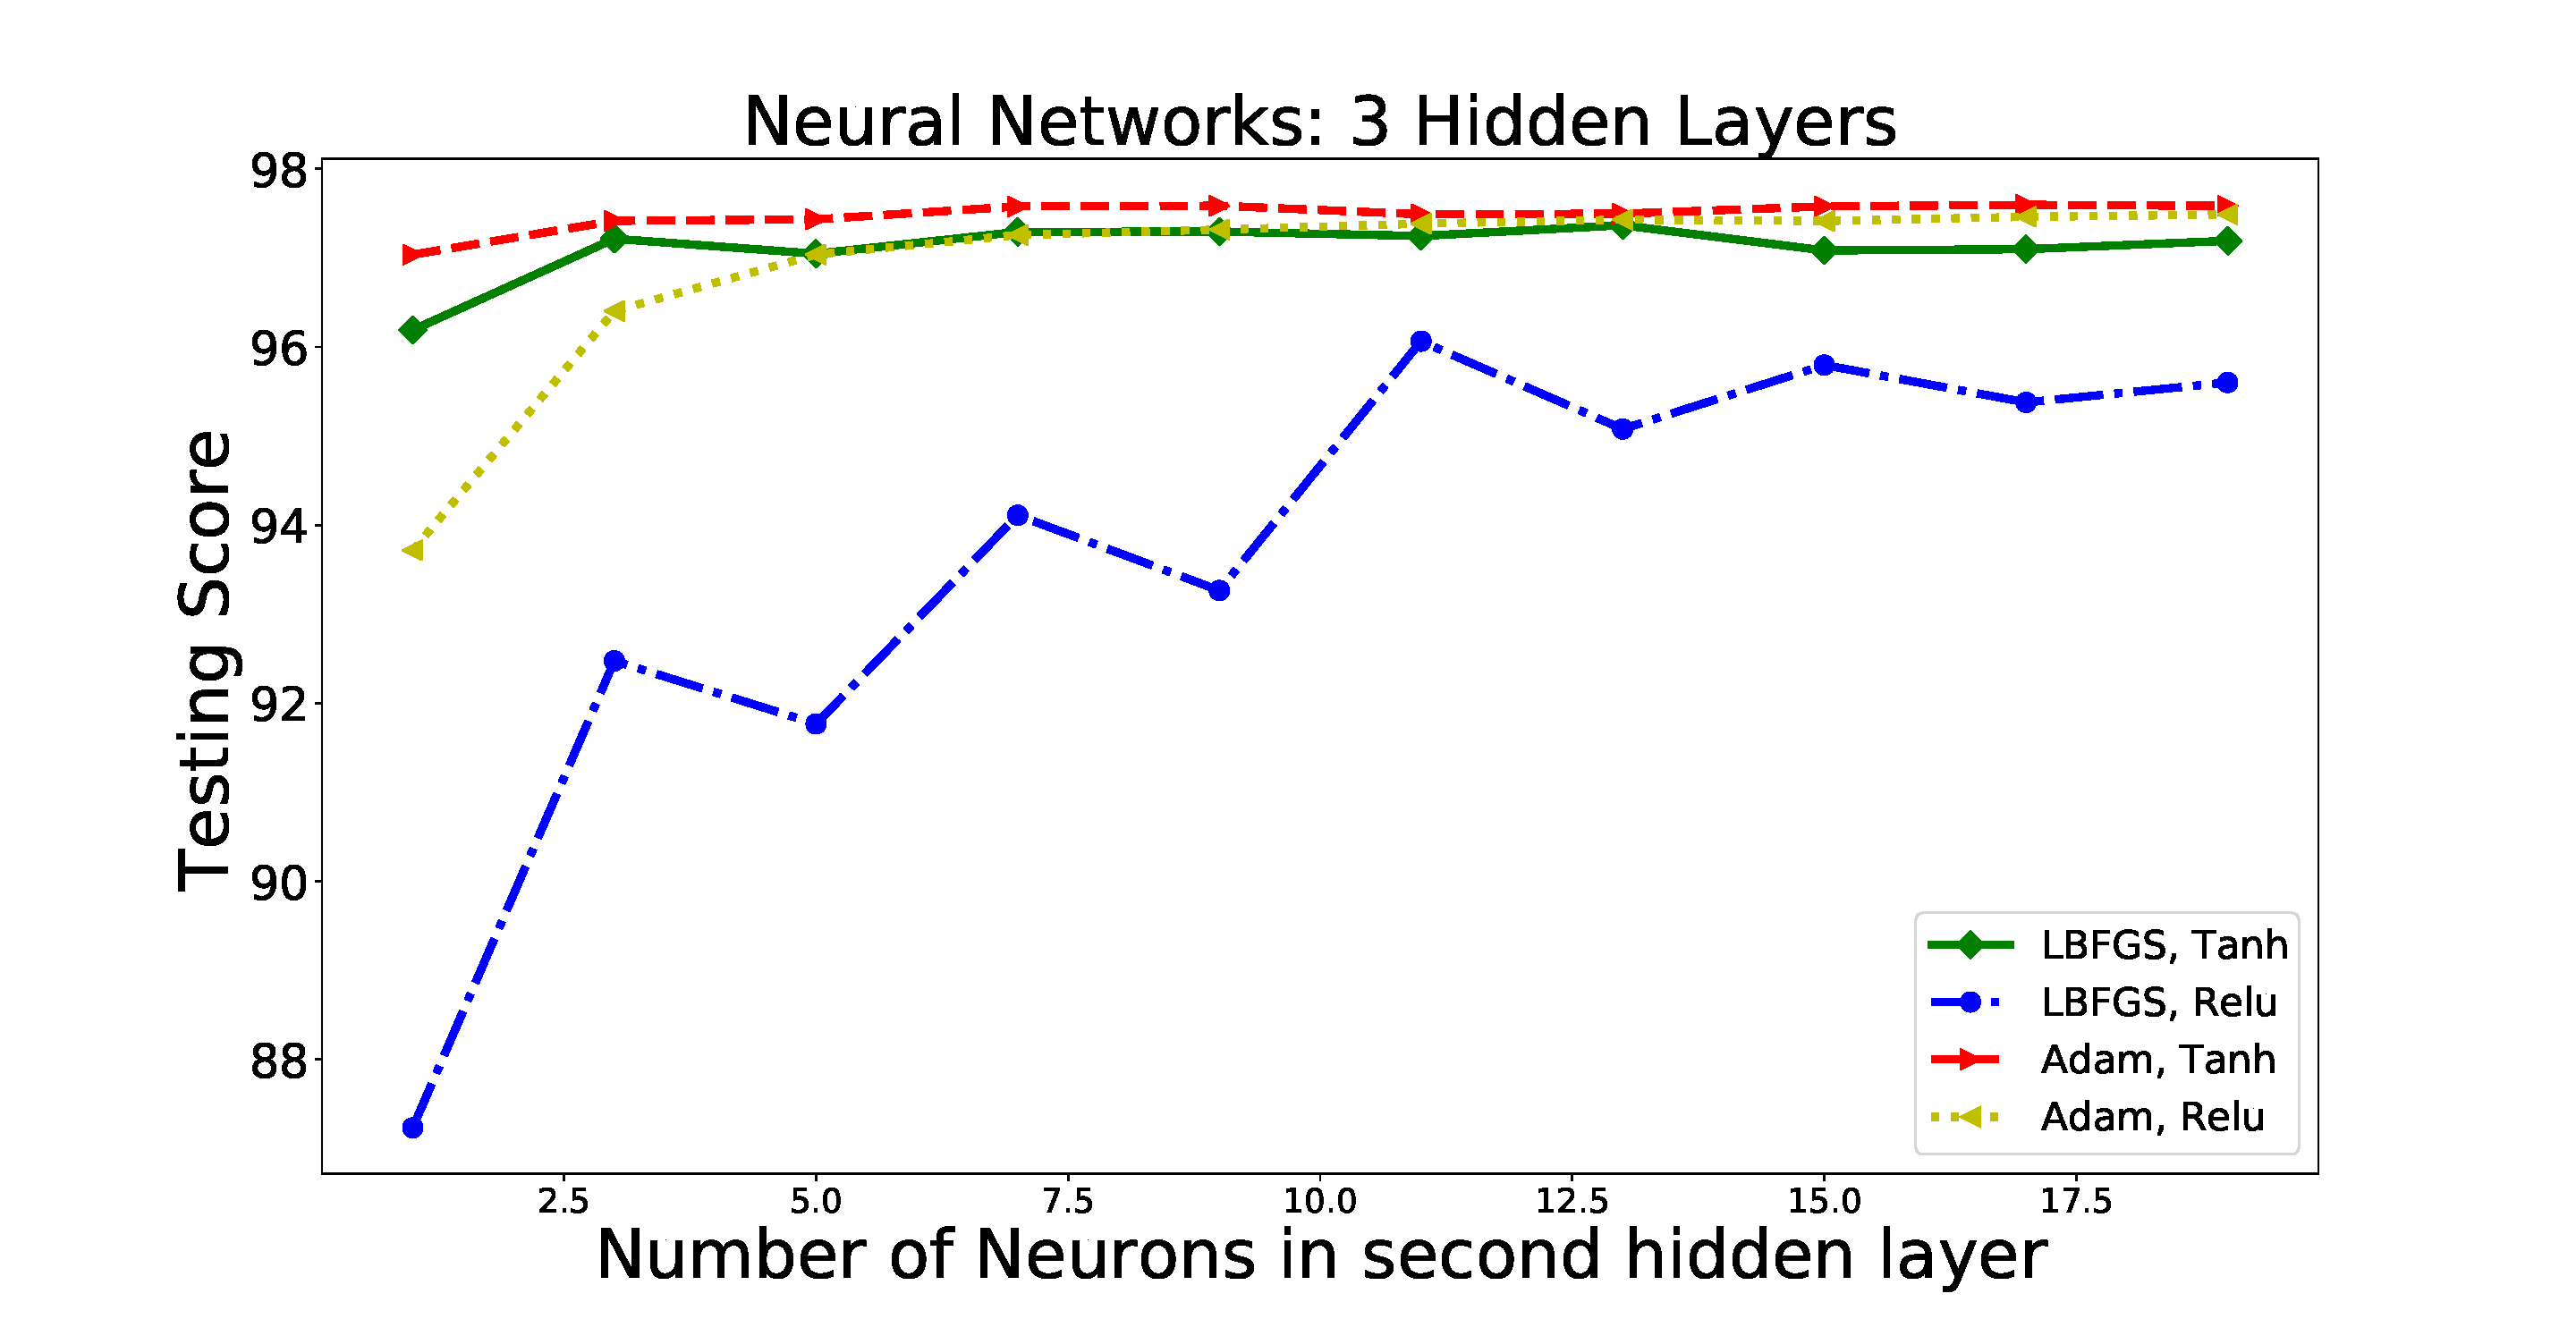
\includegraphics[width=\twopicsp\textwidth]{plots/nn_2layers_3fgl.pdf}
\caption{Dependence of NN on the number of neurons in the second hidden layer, for 11 neurons in the first hidden layer.
}
\label{fig:nn_nn}
\end{figure}


\pgfplotstableread[col sep=comma]{tables/features/3fglassocfeaturesAGNPSRnewfeats.csv}\tablea
\begin{table}
\centering
\resizebox{0.45\textwidth}{!}{
\pgfplotstabletypeset[
columns={Name,Mean,SD,Minimum,Maximum},
column type=c,
string type,
every head row/.style={before row=\hline\hline,after row=\hline,},
every last row/.append style={after row={\hline} },
every first column/.style={column type/.add={}{}},
every last column/.style={column type/.add={}{}},
columns/Name/.style={column name=Feature Name,string replace*={_}{\textunderscore}},
columns/Mean/.style={column name=Mean,column type=c,numeric type,fixed,precision=2},
columns/SD/.style={column name=Standard Deviation,numeric type,fixed,precision=2},
columns/Minimum/.style={column name=Minimum,numeric type,fixed,precision=2},
columns/Maximum/.style={column name=Maximum,numeric type,fixed,precision=2},
skip rows between index={11}{25}
]{\tablea}
}
\vspace{2mm}
\caption{Statistics of features used for 2 class probabilistic classification of the 3FGL sources.
\lb{tab:3FGL_features}}
\end{table}

\pgfplotstableread[col sep=comma]{tables/features/4fgldr2agnpsrfeatures.csv}\tableaf
\begin{table}
\centering
\resizebox{0.45\textwidth}{!}{
\pgfplotstabletypeset[
columns={Name,Mean,SD,Minimum,Maximum},
column type=c,
string type,
every head row/.style={before row=\hline\hline,after row=\hline,},
every last row/.append style={after row={\hline} },
every first column/.style={column type/.add={}{}},
every last column/.style={column type/.add={}{}},
columns/Name/.style={column name=Feature Name,string replace*={_}{\textunderscore}},
columns/Mean/.style={column name=Mean,column type=c,numeric type,fixed,precision=2},
columns/SD/.style={column name=Standard Deviation,numeric type,fixed,precision=2},
columns/Minimum/.style={column name=Minimum,numeric type,fixed,precision=2},
columns/Maximum/.style={column name=Maximum,numeric type,fixed,precision=2},
]{\tableaf}
}
\vspace{2mm}
\caption{Statistics of features used for 2 class probabilistic classification of the 4FGL-DR2 sources.
\lb{tab:4FGL_features}}
\end{table}


\begin{table}[!h]
\tiny
\centering
\renewcommand{\tabcolsep}{1mm}
\renewcommand{\arraystretch}{1}

\begin{tabular}{c c c}
\hline
\hline
Feature & RF: 50, 6& BDT: 100, 2\\
\hline
{ $\ln$(LP\_SigCurv)}&  0.297  & 0.465   \\
{LP\_beta}&0.151&0.109\\
{ $\ln$(Variability\_Index)} &0.085& 0.253   \\
$\ln$(Unc\_Energy\_Flux100)& 0.081&0.059  \\
$\ln$(Energy\_Flux100) & 0.076&0.008   \\
HR56&0.071& 0.015  \\
Unc\_LP\_Index & 0.067&0.009  \\
HR34& 0.035&0.005  \\
$\ln$(Pivot\_Energy)&0.031&0.006\\
HR23 &0.025& 0.005     \\
 LP\_Index& 0.015&0.016  \\
HR67&0.015&0.010\\
HR45&0.015&0.006\\
GLON&0.013&0.017\\
HR12&0.009&0.004\\
GLAT&0.007&0.003\\
\hline
\end{tabular}
\vspace{2mm}
\caption{Feature importances for classification of 4FGL-DR2 sources using
RF (50 trees, max depth 6) and BDT (100 trees, max depth 2) algorithms
ordered by decreasing importance 
in the case of RF algorithm.
}
\label{tab:feat_imp2}
\end{table}



We summarize features and their statistics,
which we use for probabilistic classification of sources in the 3FGL and 4FGL-DR2 catalogs
in Tables \ref{tab:3FGL_features} and \ref{tab:4FGL_features} respectively. 
We show the feature importances for the 2-class classification of 4FGL-DR2 sources in Table \ref{tab:feat_imp2}.
Similarly to feature importances for the 3FGL 2-class classification reported in Table \ref{tab:feat_imp}, 
some of the most important features are significance of curvature in the spectrum, variability index, energy flux above 100 MeV and its uncertainty.

\section{Comparison of Oversampling methods}
\lb{sec:app_O_vs_S}

In this appendix we compare the method of oversampling by repeating sources described in Section \ref{sec:oversampling} 
with SMOTE \citep{2011arXiv1106.1813C}. We use SMOTE from the Imbalanced-learn library, which is based on an implementation of \citet{Chawla_2002}. 
We estimate the probabilities of classification of all sources in the 3FGL and 4FGL-DR2 catalogs using the same algorithms and meta-parameters as in Section \ref{sec:oversampling}.
The only difference in the SMOTE case is the oversampling technique.
%SMOTE oversamples by creating synthetic data based on the data points already available. 
%For a direct comparison we used the associated sources in 3FGL/4FGL-DR2 and compared the probabilities of the individual sources. 
First, we compare the difference in class probabilities for individual sources relative to the statistical uncertainty due to the random choice of the training samples.
%We calculate normalized differences of individiual probabilities $P_{D}$ by the formula:
In particular, we calculate the difference of probabilities to belong to, e.g., PSR class relative to the maximal standard deviation
between the oversampling-by-repeating and SMOTE

\be
\lb{eq:OS_diff}
\Delta = \frac{P_O - P_S}{max(\sigma_{O},\sigma_{S})},
\ee
where $P_O$ ($P_S$) is the probability for the oversampling-by-repeating (SMOTE) and $\sigma_O$ ($\sigma_S$) is the corresponding standard deviation. 
The mean and the standard deviation of $\Delta$ for 2- and 3-class cases in the 3FGL and 4FGL-DR2 catalogs are presented in 
Tables \ref{tab:OvsS_3FGL} and \ref{tab:OvsS_4FGL} respectively.
We note that in the 3-class case we use less oversampling than in the 2-class case, namely, the oversampling factor in the 3-class case is equal to the square root of the ratio of the number of sources, while in the 2-class case it is equal to the ratio of the number of associated AGNs to the number of associated pulsars.
This is the reason for the smaller bias and standard deviation of the difference in the 3-class case relative to the 2-class case.
Overall, the differences for individual probabilities are smaller than the uncertainties due to randomness of training.

\begin{table}[!h]
\tiny
\centering
\renewcommand{\tabcolsep}{1mm}
\renewcommand{\arraystretch}{1.3}

\begin{tabular}{c c c c c }
\hline
\hline
Classes&\multicolumn{2}{c}{2-Class}&\multicolumn{2}{c}{3-Class}\\
Method & Mean&Std.&Mean&Std.\\
\hline
RF& -0.431 & 0.461&0.114&0.343\\
\hline
BDT&-0.161&0.426 &-0.102&0.337\\
\hline
NN&0.285&0.419&0.224&0.254\\
\hline
LR&0.437&0.615&0.357&0.325\\
\end{tabular}
\vspace{2mm}
\caption{The parameters of the distribution of $\Delta$ in Eq.  (\ref{eq:OS_diff})
for the 4 algorithms used in 3FGL with PSR-like probabilities for all sources.
}
\label{tab:OvsS_3FGL}
\end{table}





\begin{table}[!h]
\tiny
\centering
\renewcommand{\tabcolsep}{1mm}
\renewcommand{\arraystretch}{1.3}

\begin{tabular}{c c c c c}
\hline
\hline
Classes&\multicolumn{2}{c}{2-Class}&\multicolumn{2}{c}{3-Class}\\
Method & Mean&Std.&Mean&Std.\\
\hline
RF& -0.335 & 0.489&-0.491&0.464\\
\hline
BDT&-0.120&0.581 &0.007&0.423\\
\hline
NN&0.472&0.430&0.171&0.145\\
\hline
LR&0.531&0.732&0.347&370\\
\end{tabular}
\vspace{2mm}
\caption{The parameters of the distribution of $\Delta$ in Eq.  (\ref{eq:OS_diff})
for the 4 algorithms used in 4FGL-DR2 with PSR-like probabilities for all sources.
}
\label{tab:OvsS_4FGL}
\end{table}

The LR algorithm has some of the largest differences.
We plot the histogram of the $\Delta$ for the PSR-like probabilities in the 3FGL (4FGL-DR2) catalogs in Fig. \ref{fig:OvsS_3FGL_PSR}
(\ref{fig:OvsS_4FGL_PSR}).

\begin{figure}[h]
\centering
\hspace*{-0.5cm}
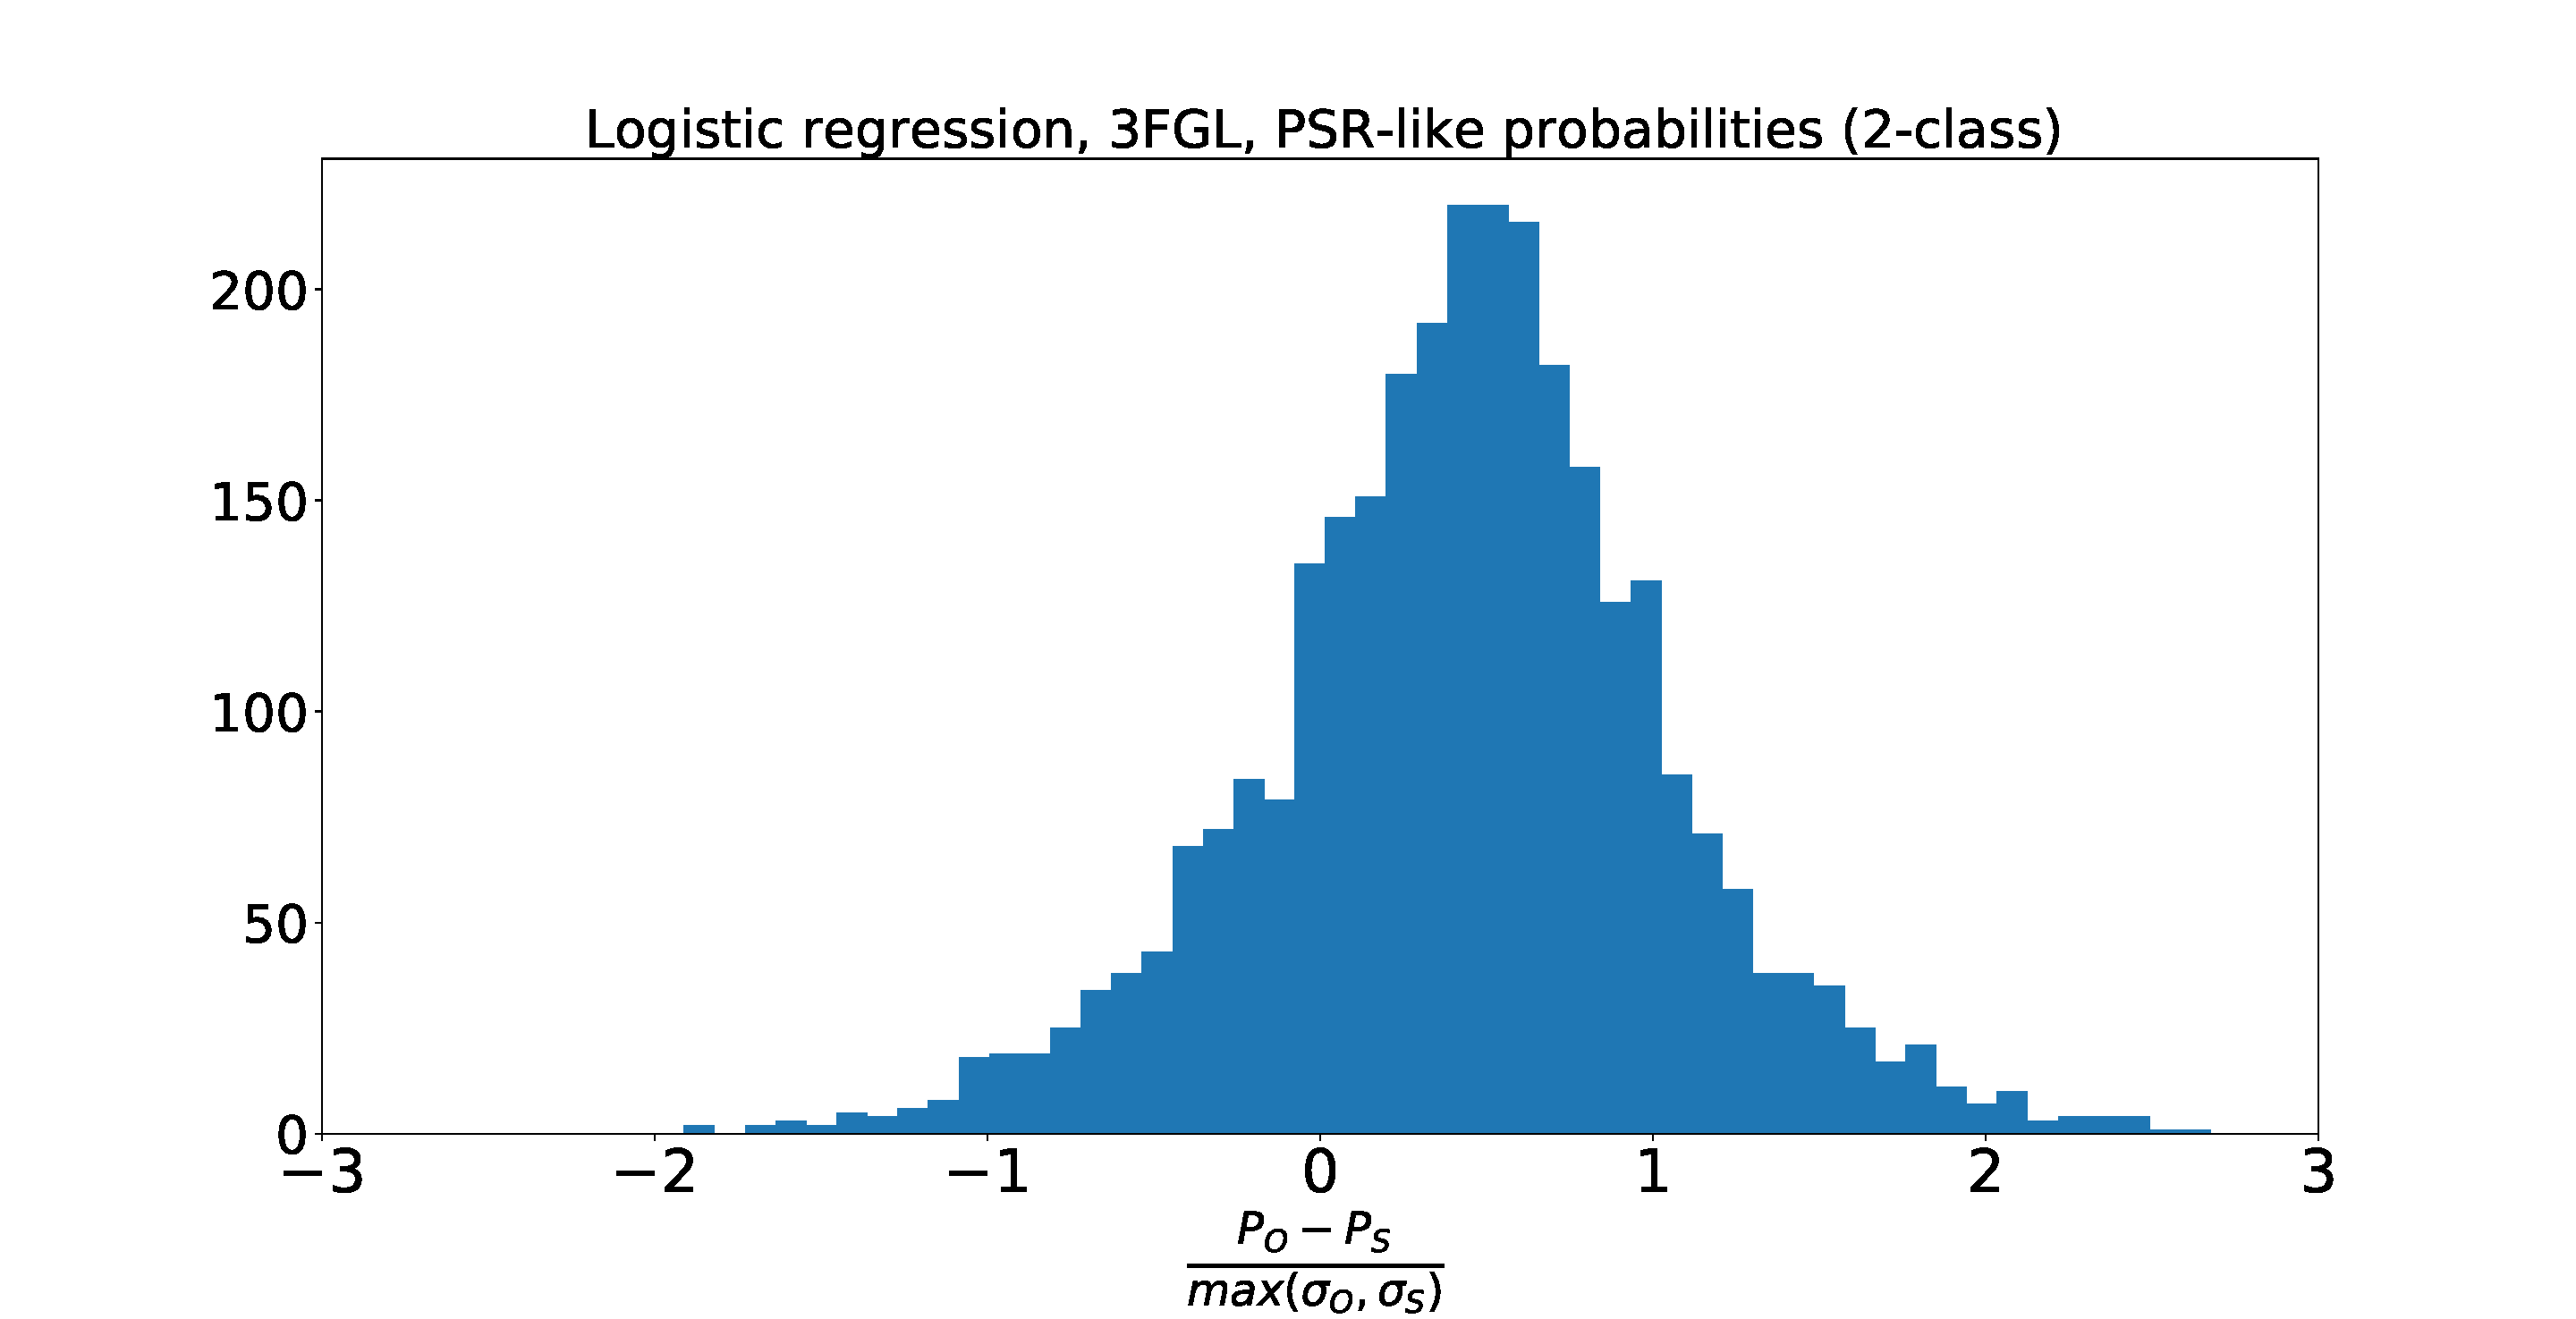
\includegraphics[width=0.55\textwidth]{plots/hist_diff_smote_LR_3FGL_2class.pdf}
\hspace*{-0.5cm}
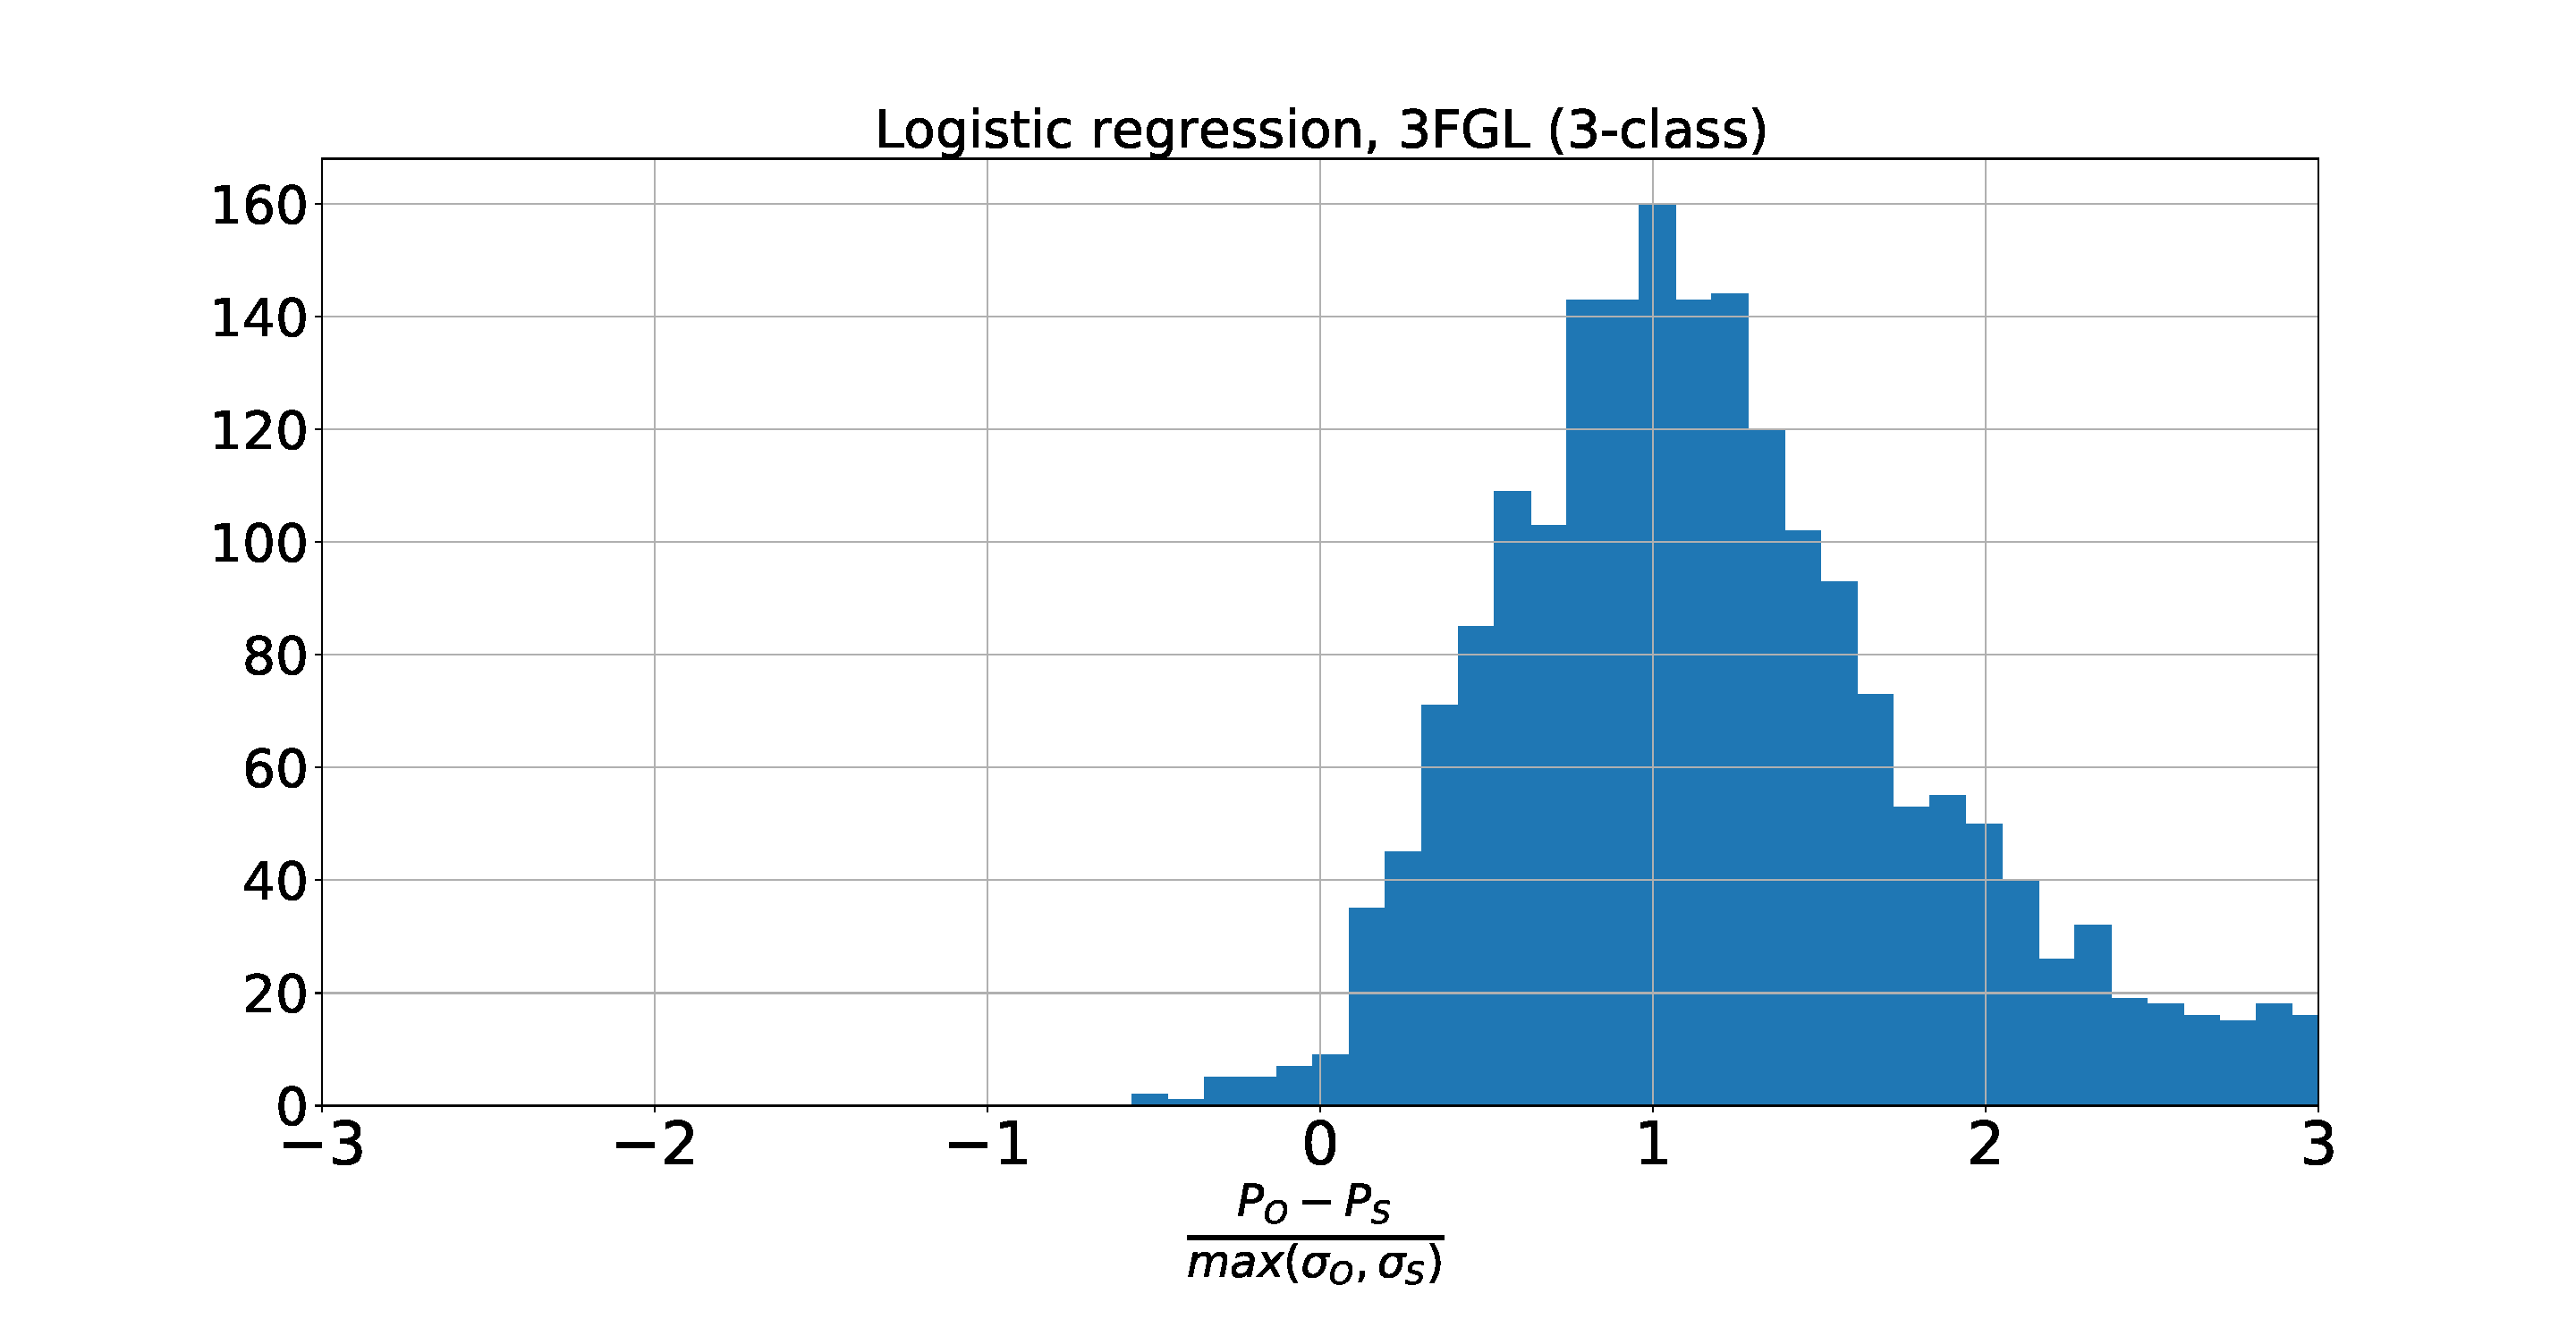
\includegraphics[width=0.55\textwidth]{plots/hist_diff_smote_LR_3FGL_3class.pdf}
\caption{Distribution of difference  of probabilities derived with oversampling-by-repeating ($P_O$) and SMOTE ($P_S$) 
relative to the standard deviations due to random choice of training samples
for LR in the 2-class (top) and the 3-class (bottom) classifications of the 3FGL sources.
}
\label{fig:OvsS_3FGL_PSR}
\end{figure}

\begin{figure}[h]
\centering
\hspace*{-0.5cm}
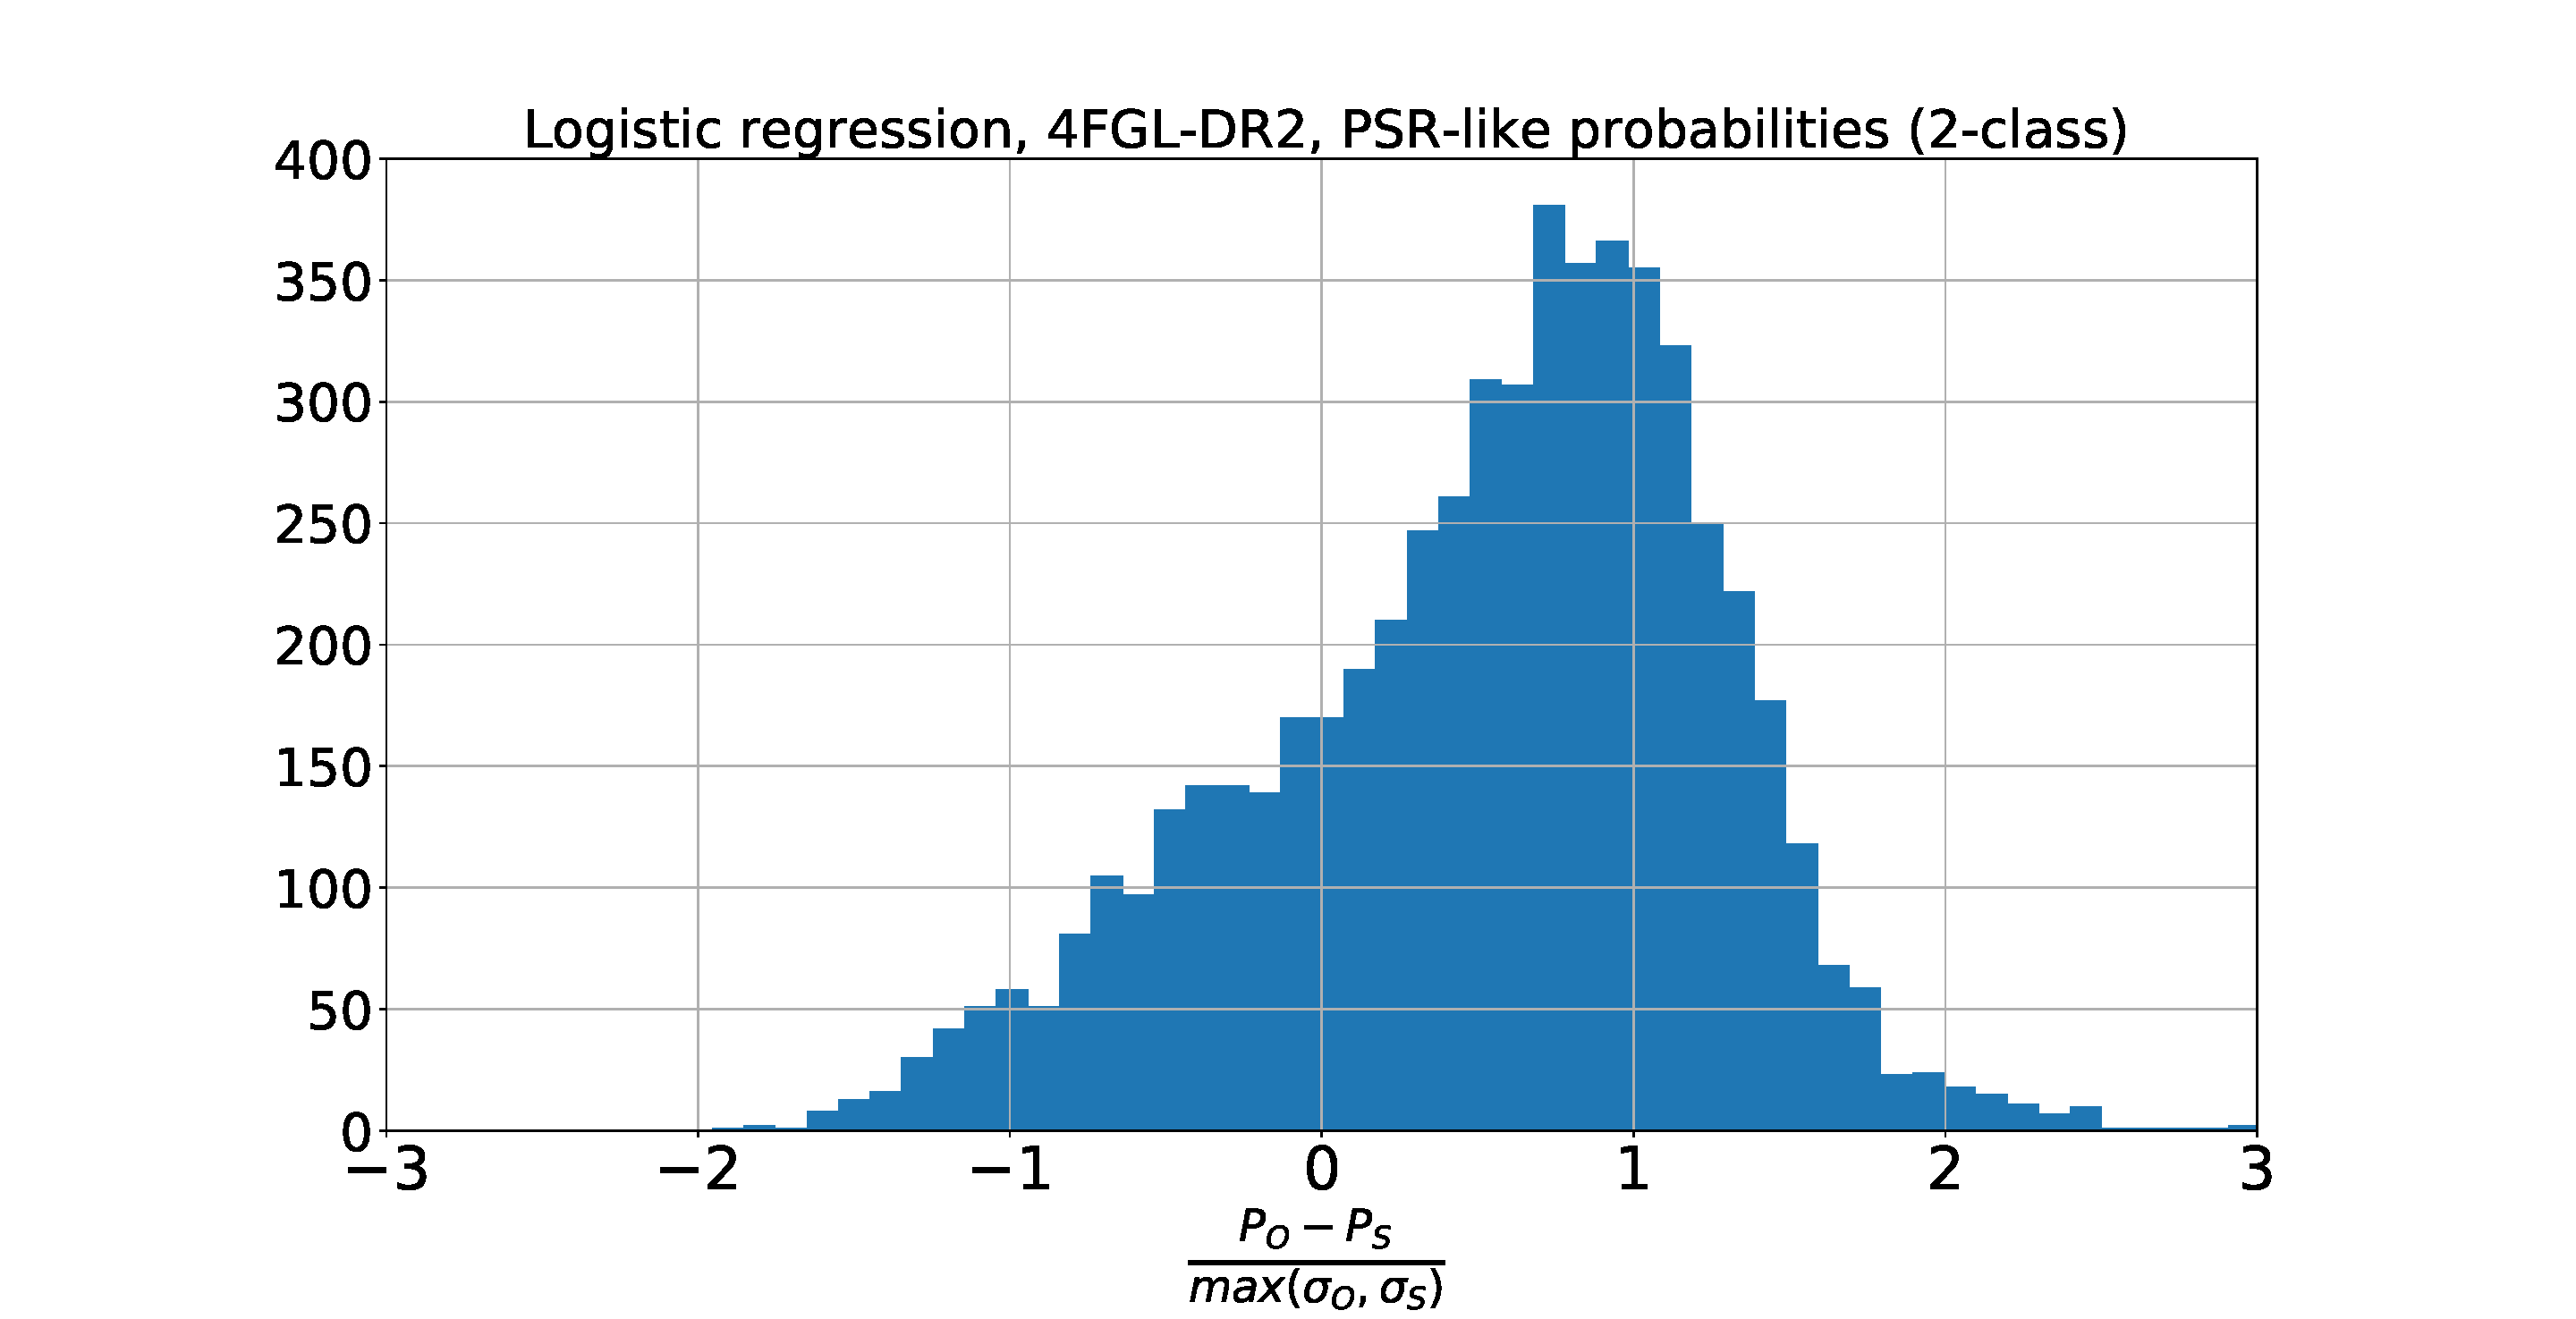
\includegraphics[width=0.55\textwidth]{plots/hist_diff_smote_LR_4FGL-DR2_2class.pdf}
\hspace*{-0.5cm}
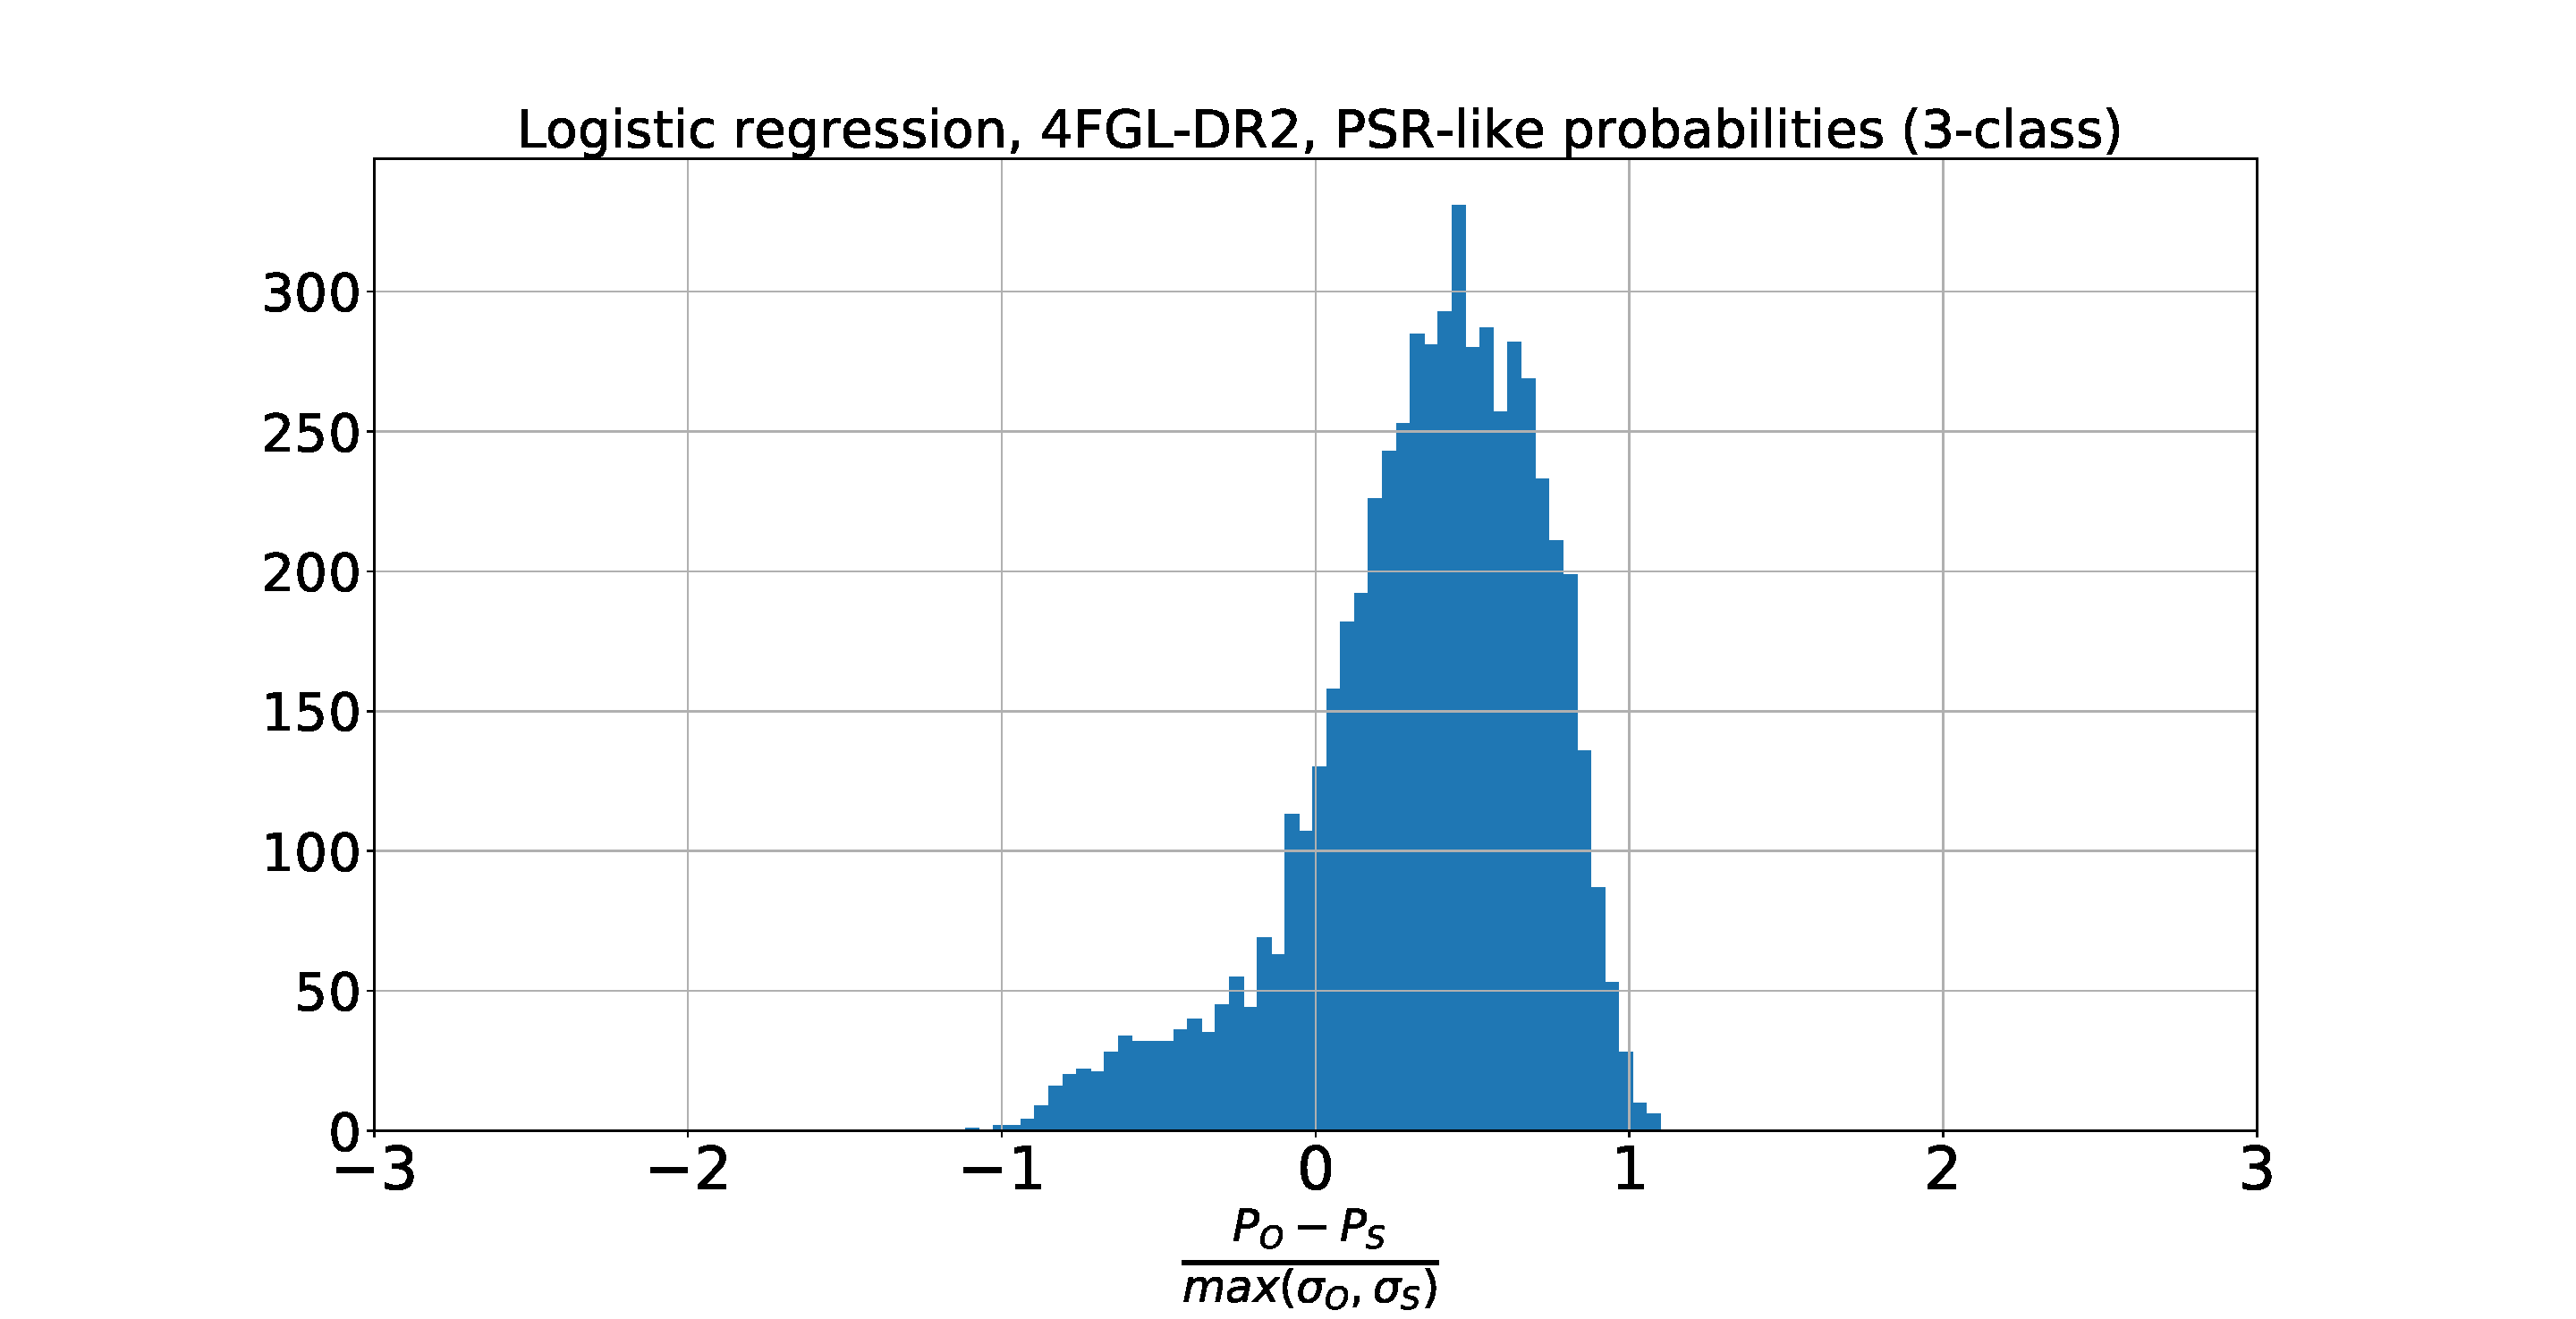
\includegraphics[width=0.55\textwidth]{plots/hist_diff_smote_LR_4FGL-DR2_3class.pdf}
\caption{Same as Fig. \ref{fig:OvsS_3FGL_PSR} for the 4FGL-DR2 catalog.
}
\label{fig:OvsS_4FGL_PSR}
\end{figure}


The difference between oversampling-by-repeating and SMOTE is illustrated in Fig. \ref{fig:domains_smote_over}.
The domains are determined by averaging over 100 random choices of the training data.
One of these choices is shown on the plots: in this case, both oversampling-by-repeating and SMOTE have the same 
training and testing samples.
In the oversampling-by-repeating the training sources are oversampled by simply repeating the sources,
while in SMOTE new sources are created by randomly placing sources in the parameter space along the lines connecting a source
and one of its nearest neighbours. In our implementation we choose one out of the 5 nearest neighbours. 


\begin{figure}[h]
\centering
%\hspace*{-0.5cm}
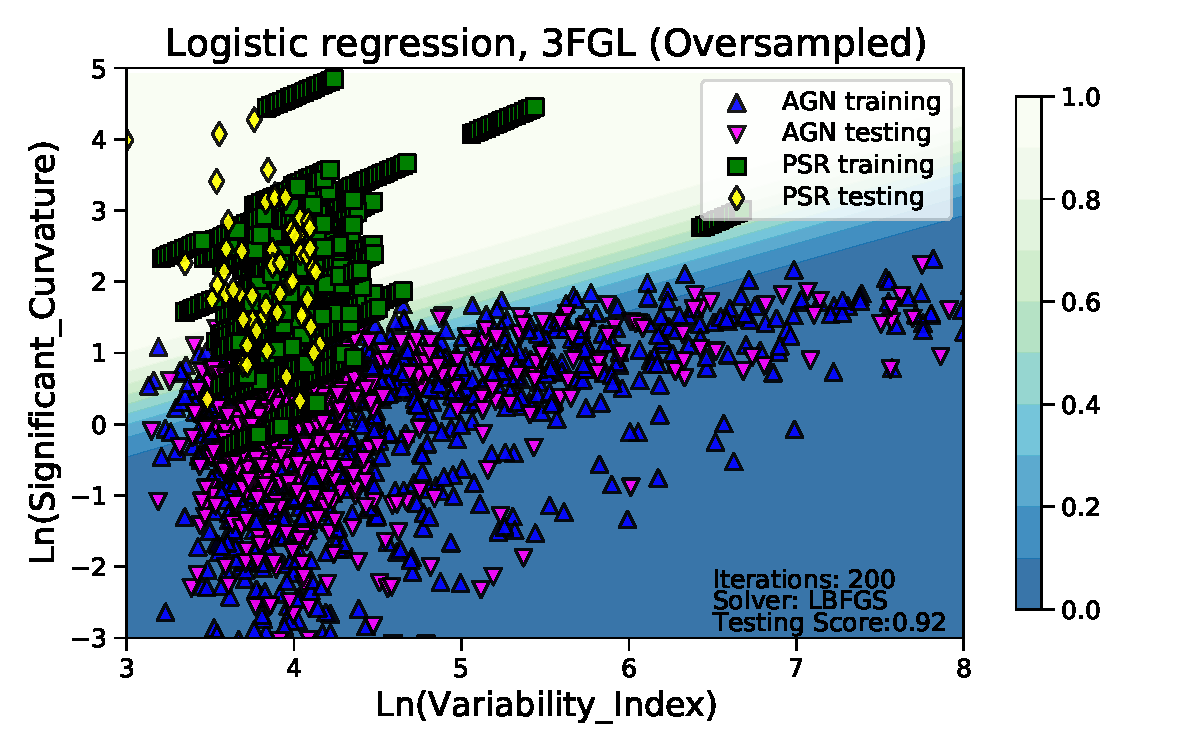
\includegraphics[width=0.55\textwidth]{plots/classification_domains/domains_oversampled_LR_3FGL_2class.pdf}
%\hspace*{-0.5cm}
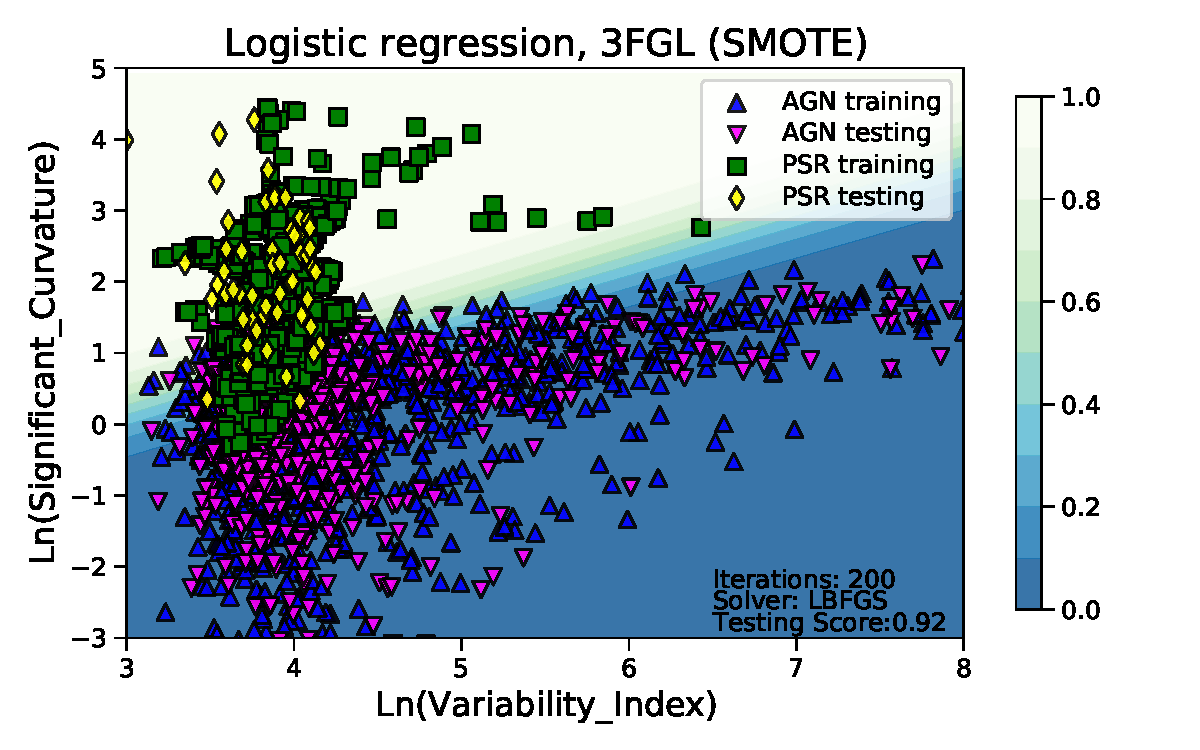
\includegraphics[width=0.55\textwidth]{plots/classification_domains/domains_smote_LR_3FGL_2class.pdf}
\caption{Comparison of classification domains for the 2-class classification of the 3FGL sources
using LR with oversampling by repeating sources (top) and SMOTE (bottom).
}
\label{fig:domains_smote_over}
\end{figure}


Although the mean and the standard deviations for the probabilities of the individual sources are smaller than the 
statistical uncertainties of the probabilities, the presence of the bias can have a significant effect when we sum the probabilities, e.g., in population studies.
In order to check this effect we compare the source count distributions as a function of flux for oversampling-by-repeating and SMOTE 
in Fig. \ref{fig:S_vs_O_NlogS}.
We show the expected number of pulsars among unassociated sources for the 2- and 3-class cases using the 3FGL and 4FGL-DR2 catalogs.
We also show the expected number of OTHER sources in the 3-class case.
The difference can indeed be significant for some of the algorithms, but the change is comparable or smaller than the difference among the algorithms.
The classification probabilities in the 2- and 3-class cases with SMOTE for the 3FGL and 4FGL-DR2 catalogs 
are available online in the SOM/SMOTE subfolder in the supplementary online materials \citep{SOM_material}.

\begin{figure*}[h]
\centering
\hspace*{-0.5cm}
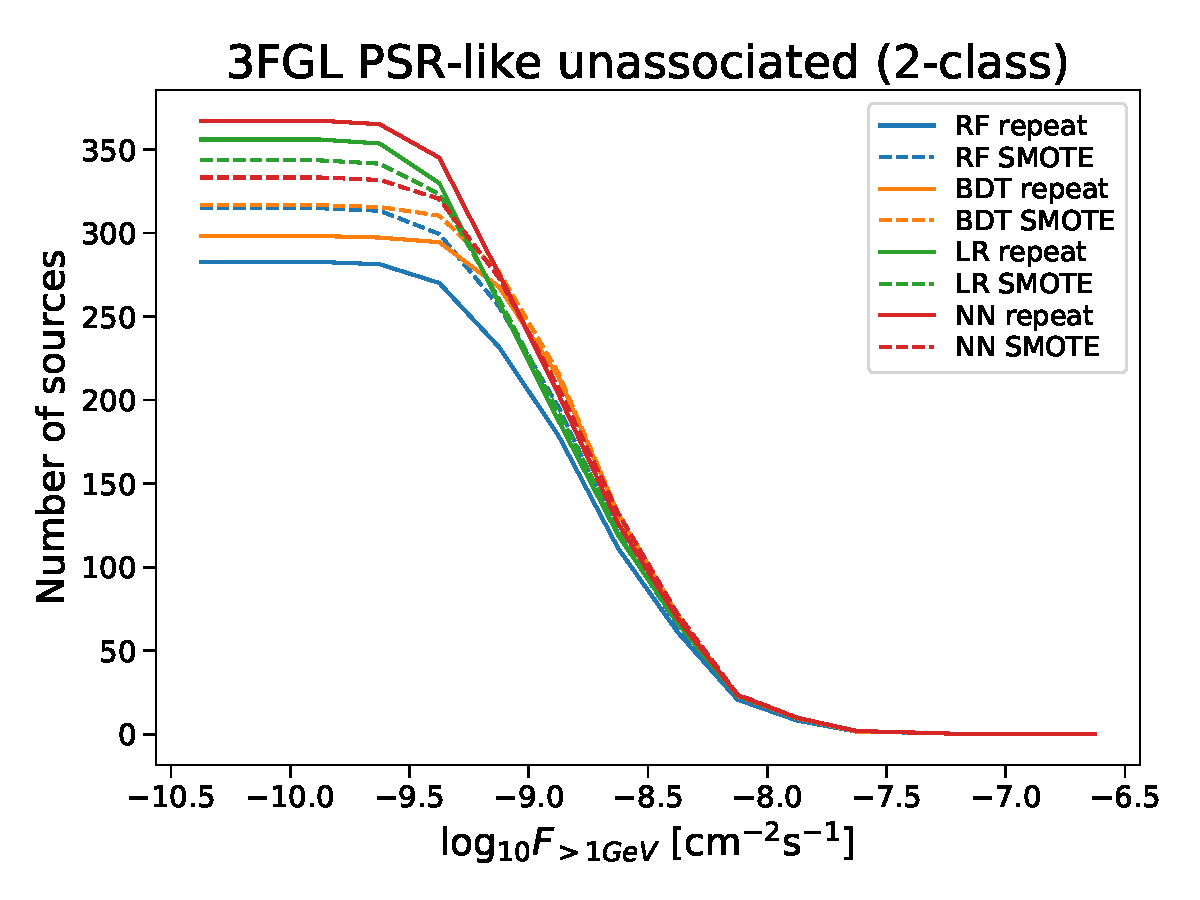
\includegraphics[width=0.45\textwidth]{plots/oversample/N_logS_3FGL_PSR_2classes_O_vs_S.pdf}
\hspace*{-0.5cm}
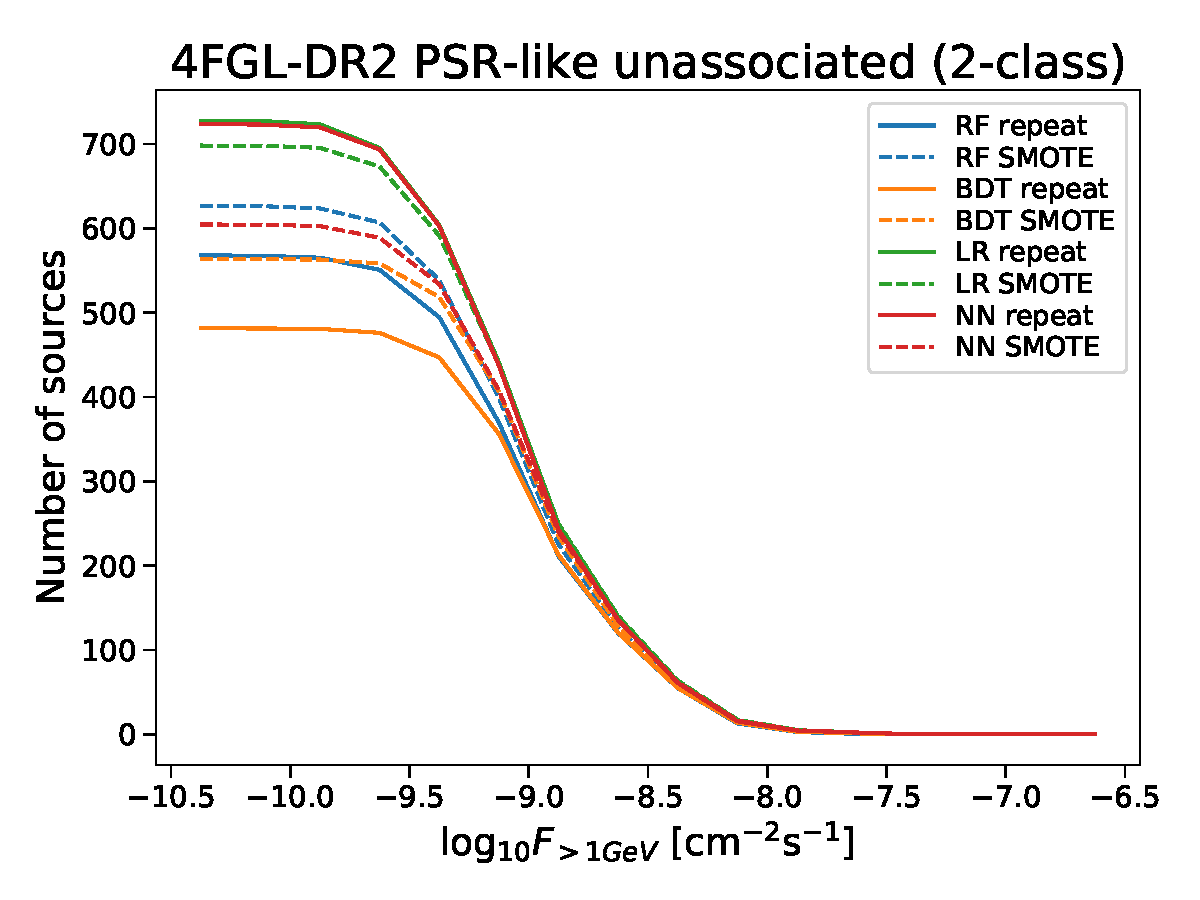
\includegraphics[width=0.45\textwidth]{plots/oversample/N_logS_4FGL-DR2_PSR_2classes_O_vs_S.pdf}\\
\hspace*{-0.5cm}
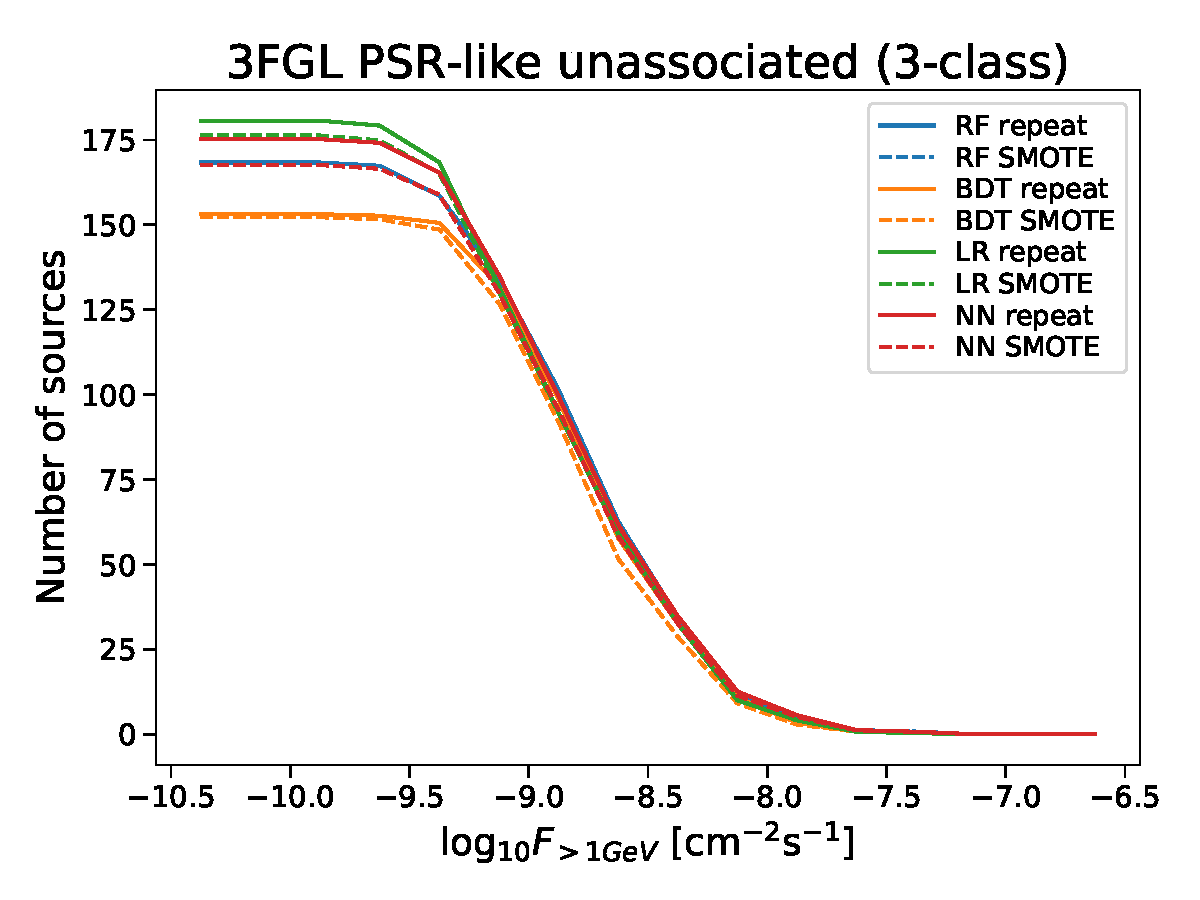
\includegraphics[width=0.45\textwidth]{plots/oversample/N_logS_3FGL_PSR_3classes_O_vs_S.pdf}
\hspace*{-0.5cm}
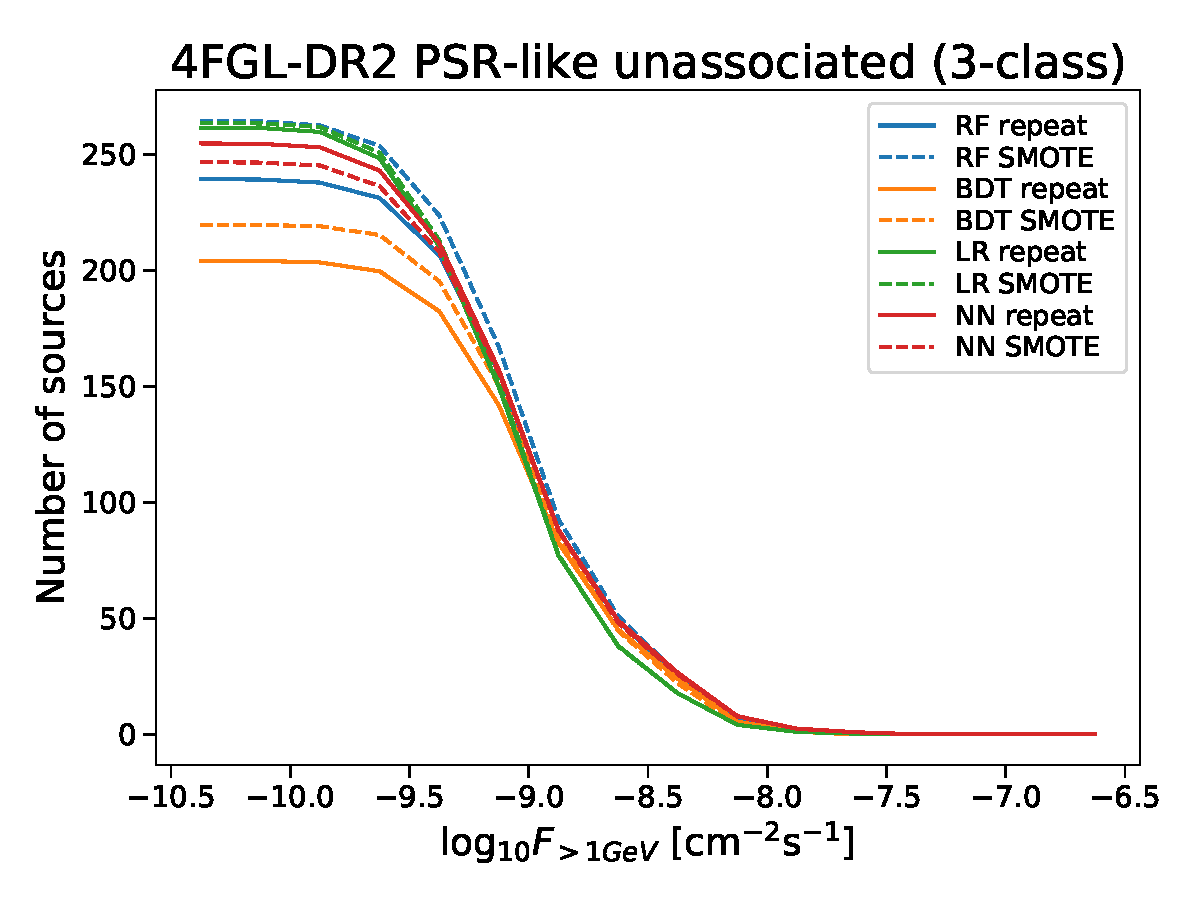
\includegraphics[width=0.45\textwidth]{plots/oversample/N_logS_4FGL-DR2_PSR_3classes_O_vs_S.pdf}\\
\hspace*{-0.5cm}
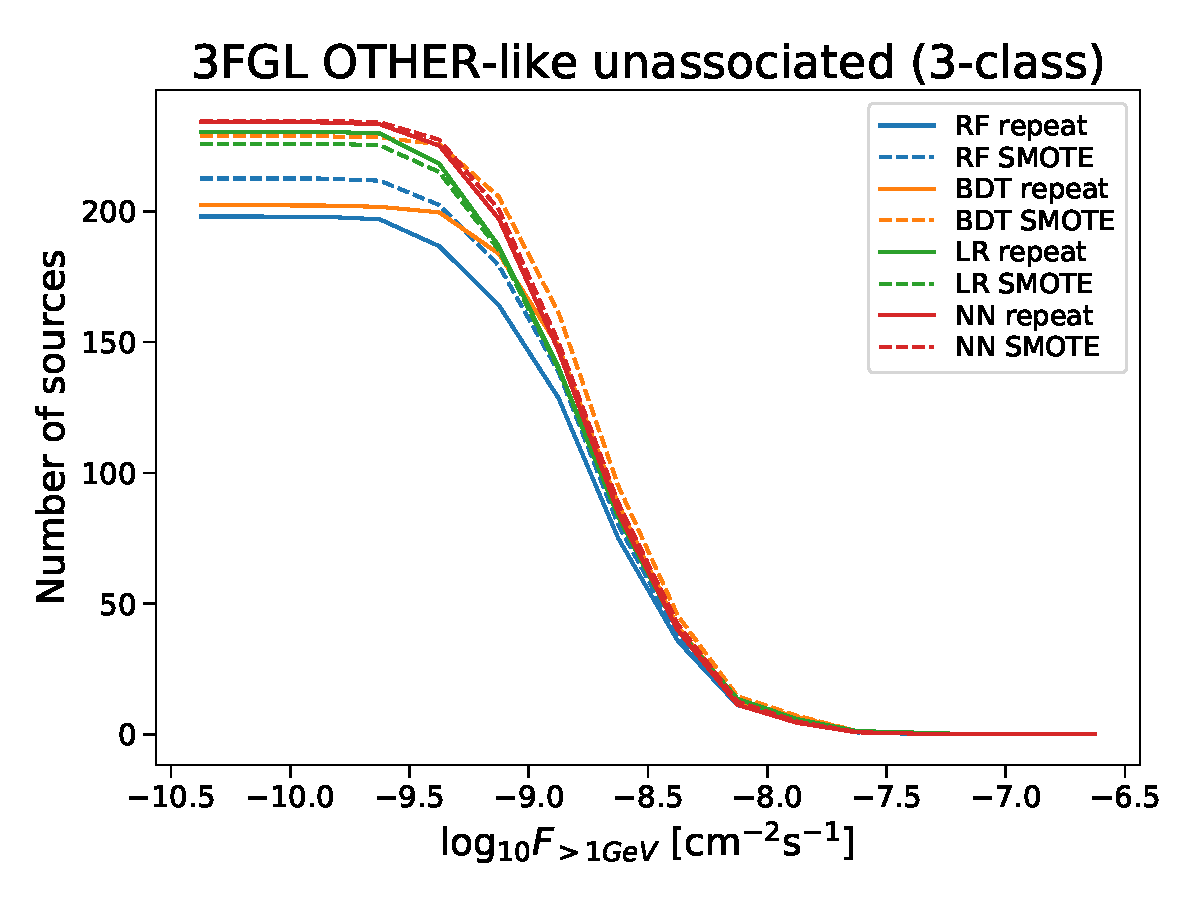
\includegraphics[width=0.45\textwidth]{plots/oversample/N_logS_3FGL_OTHER_3classes_O_vs_S.pdf}
\hspace*{-0.5cm}
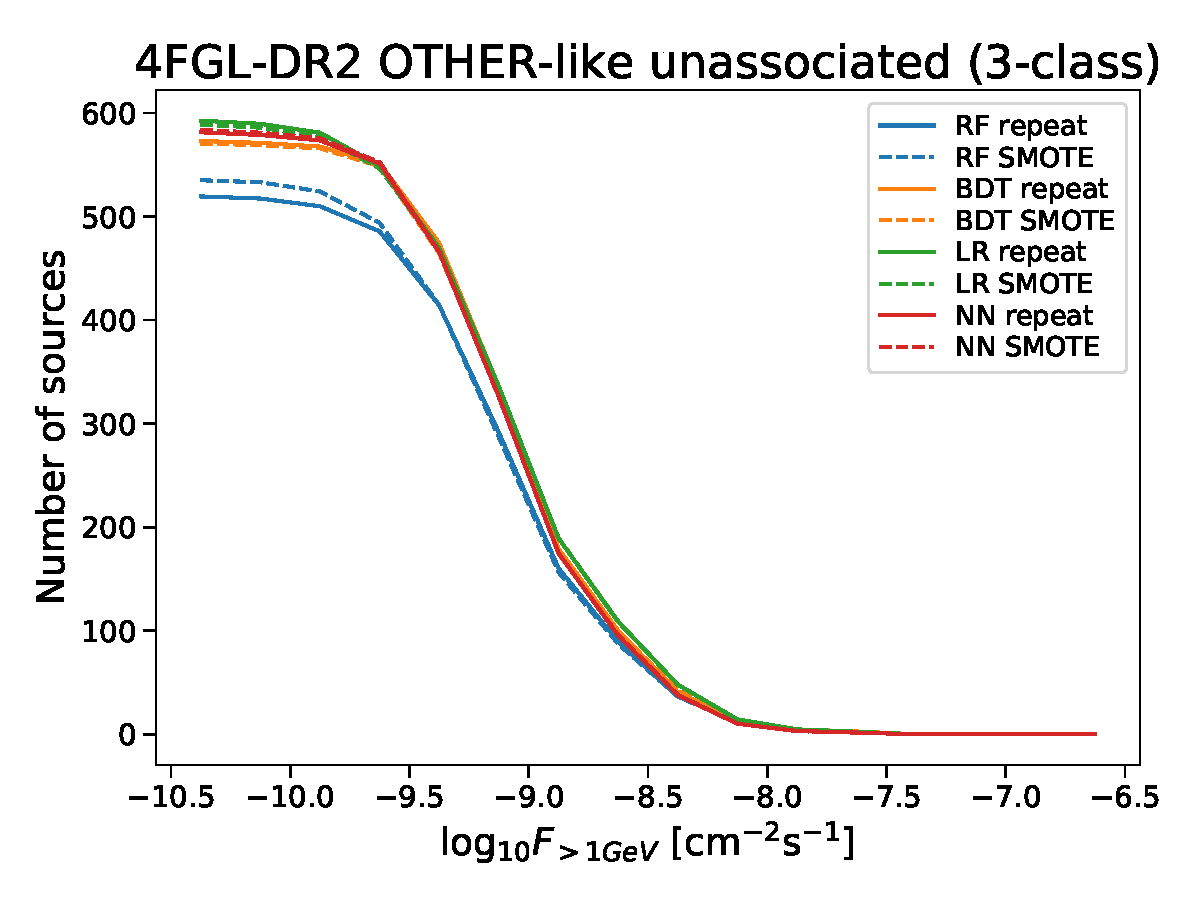
\includegraphics[width=0.45\textwidth]{plots/oversample/N_logS_4FGL-DR2_OTHER_3classes_O_vs_S.pdf}
\caption{Comparison of source count distributions as a function of flux for the estimated number of PSR and OTHER sources
among the unassociated sources in the 2- and 3-class cases for oversampling-by-repeating and SMOTE.
The number of PSR-like sources in the 2-class case is not corrected for the presence of OTHER sources.
The changes due to using SMOTE oversampling technique are comparable to the difference among the algorithms
for oversampling by repeating.
}
\label{fig:S_vs_O_NlogS}
\end{figure*}
